% dsilab_monograph_en.tex — the DSI laboratory monograph (English edition)
\documentclass[11pt,a4paper]{article}
\usepackage[margin=2.4cm]{geometry}
\usepackage{amsmath,amssymb,amsthm}
\usepackage{booktabs}
\usepackage{graphicx}
\usepackage{xcolor}
\usepackage[colorlinks=true,linkcolor=blue!60!black,urlcolor=blue!60!black,citecolor=blue!60!black]{hyperref}
\usepackage{caption}
\captionsetup{font=small,labelfont=bf}

\newtheorem{theorem}{Theorem}
\newtheorem{lemma}[theorem]{Lemma}
\newtheorem{corollary}[theorem]{Corollary}
\theoremstyle{definition}
\newtheorem{definition}[theorem]{Definition}
\newcommand{\F}{\mathrm{F}}
\newcommand{\norm}[1]{\lVert #1\rVert}

\title{\bf The DSI Laboratory:\\ Dynamics of Invariants for the $b$--C/$a$--C Framework\\
\large Seven deterministic experiments on the Klein quartic, the Kunz defect\\ and the Choptuik problem --- theorem layer, census attack, honest verdicts}
\author{Ishak Khamzatovich Isaev\\ \small Nalchik, Kabardino-Balkarian Republic, Russian Federation\\[-2pt]
\small \texttt{dsi\_lab} package, version 2.0.0}
\date{October 12, 2026}

\begin{document}
\maketitle

\begin{abstract}
\noindent
The DSI laboratory (\texttt{dsi\_lab}) is a self-contained package of
seven deterministic experiments on the open problems of the
$b$--C/$a$--C spinor-correction framework. This monograph is its
theorem layer. Three results define it. (i)~\emph{The sharp trace
theorem}: the Kunz defect obeys $\F \ge 5n/7$ for every $n$, so the
framework's dream value $e = 0$ is unreachable even in principle; the
equality case is a scalar pair that fails to be a partial isometry.
(ii)~\emph{The partial-isometry theorems A/B/C}: on the class of
carrier-isometric models the floor rises to $e \ge 1$ (theorem~A), the
coverage arithmetic is exact, $\F = n + 2\,\mathrm{rank}(\mathrm{I}-P-Q)$
(theorem~B), and unitary pairs sit at $\F = 2n$ (theorem~C); the trimmed
Kunz tree attains $\F = n+2$ exactly --- the almost-extremal pair. The
sofic $\sqrt{\varepsilon}$-law is \emph{refuted} by the data.
(iii)~\emph{The census attack on DSI-4}: the last empirical input
$c_{K3}$ matches $9/224 = 27/672$ to $+0.0025\%$, the denominator
$224 = 4\cdot 56$ is generated by the $\{7,3\}$ tiling of the Klein
quartic, and the uniqueness lemma makes the match single out $9/224$
among all census-legal fractions. Two corrections were \emph{produced
by} the package and are kept as first-class results: finding~D1 (the
genus-14 Hurwitz row is impossible; the correct group is
$\mathrm{PSL}(2,13)$) and finding~E1 (the trace identity of the QCD
bridge exists only after centering $\langle\lambda\rangle$). Every
claim carries a status --- proved, verified numerically, refuted, or
hypothesis --- and an address in the claim ledger. The exact stratum of
the theorem layer is formalized in Lean~4 (sorry-free); theorems
A/B/C are axiom-anchored to 24{,}000 machine-verified pairs with
identity error $5.9\cdot 10^{-16}$.
\end{abstract}

\tableofcontents

\section{Introduction}\label{sec:intro}

The parent repository verifies two spinor corrections --- the
first-order Berry-type $b$--C and the second-order braking $a$--C --- on
the Klein quartic curve, with the unified Choptuik formula built on the
septinial phase $\delta_C = \pi/7$. Every quantity of the framework is
dimensionless, and the discipline of the verification programme is
honesty: proved, verified and refuted are never mixed.

The DSI laboratory asks a harder question: \emph{which inputs of the
framework can survive without being assumed?} It answers with seven
deterministic experiments (table~\ref{tab:experiments}), each
reproducible byte-for-byte with fixed seeds, each leaving its verdict
in a committed JSON file.

\begin{table}[ht]
\centering\small
\begin{tabular}{@{}clp{7.2cm}@{}}
\toprule
\# & experiment & verdict \\
\midrule
1 & \texttt{exp1\_sh3\_bridge} & trace bridge Sh.3(iii): the sharp theorem confirmed ($n=7..12$, gap $\le 5.9\cdot10^{-8}$); the Cuntz tree $\F = n+2$ exact; the sofic $\sqrt{\varepsilon}$-law \textbf{refuted} \\
2 & \texttt{exp2\_dsi4} & DSI-4: $c_{K3} = 27/672 = 9/224$; convergent of rank \#1 for $q \le 2000$ \\
3 & \texttt{exp3\_hurwitz} & finding \textbf{D1}: the repository row $(g{=}14, n{=}11)$ is impossible; $\mathrm{PSL}(2,13)$; $\Delta_{Ch}(\pi/13) = 3.3672$ \\
4 & \texttt{exp4\_qnm} & QNM catalogue: 10 events; $|\Delta f_n|/f_n = 8.3857\cdot 10^{-5}$, falsifiable; $0.84\sigma$ at Cosmic Explorer \\
5 & \texttt{exp5\_qcd} & finding \textbf{E1}: $\mathrm{tr}(Q_{K3}\oplus M_F) = 32$ requires centering; slope $-0.99$ ($\sim 1/N$); BF(GUE) up to 1165 \\
6 & \texttt{exp6\_census\_224} & why $224 = 4\cdot 56$: explicit $\{7,3\}$ census from $\mathrm{GL}(3,2)$; uniqueness lemma; degeneracy theorem \\
7 & \texttt{exp7\_e1\_threshold} & theorems A/B/C proved and verified (identity $5.9\cdot 10^{-16}$ over 24{,}000 pairs); the ladder $5/7 \to 1 \to 2$ is a theorem \\
\bottomrule
\end{tabular}
\caption{The seven experiments and their verdicts.}
\label{tab:experiments}
\end{table}

The monograph follows the theorem layer (section~\ref{sec:theorems}),
the census attack (section~\ref{sec:census}), the two corrections
(section~\ref{sec:findings}), the honesty discipline
(section~\ref{sec:honesty}) and the formalization
(section~\ref{sec:lean}).

\section{The framework and the Klein quartic}\label{sec:framework}

The septinial phase $\delta_C = \pi/7$ produces the framework constant
\[
b_{Ch} = 1-\cos(2\pi/7) = 0.37651019814126640,
\]
and the universal curve $\Delta_{Ch}(\delta) = \lambda_{D2} +
\delta^2/2 - \delta^5/22$ with $\lambda_{D2} = 3.338$. The Klein
quartic $x^3y + y^3z + z^3x = 0$ is the genus-3 curve with automorphism
group $\mathrm{PSL}(2,7) \cong \mathrm{GL}(3,2)$ of order $168$, and
its $\{7,3\}$ tiling carries the combinatorics of everything below:
$V = 56$ triangular faces, $E = 84$ edges, $F = 24$ heptagons, with the
valence identity
\begin{equation}
7F = 3V = 2E = |\mathrm{PSL}(2,7)| = 168,
\qquad V-E+F = 2-2\cdot 3 = -4.
\label{eq:census}
\end{equation}
Experiment 6 builds \eqref{eq:census} explicitly: vertices, edges and
faces are coset spaces of $G = \mathrm{GL}(3,2)$ by the stabilizers of
a point, an edge and a heptagon, and the identity is a theorem about
group orders.

\section{The Kunz defect and the theorem layer}\label{sec:theorems}

\begin{definition}
For $X_1, X_2 \in M_n(\mathbb{C})$ the \emph{Kunz defect} is
\[
\F(X_1,X_2) = \norm{X_1^*X_1-\mathrm{I}}^2 + \norm{X_2^*X_2-\mathrm{I}}^2
+ \norm{X_1^*X_2}^2 + \norm{X_1X_1^* + X_2X_2^* - \mathrm{I}}^2 ,
\]
with $\norm{\cdot}$ the Frobenius norm, and $e = \F/n$.
\end{definition}

\subsection{The sharp trace theorem}

\begin{theorem}[sharp trace theorem]\label{thm:trace}
For every $n$ and all $X_1, X_2 \in M_n(\mathbb{C})$,
$\F(X_1,X_2) \ge 5n/7$. Equality holds exactly for the scalar pair
$X_1 = X_2 = \sqrt{4/7}\,\mathrm{I}$, which is not a partial isometry.
\end{theorem}

Numerically, L-BFGS minimization with restarts lands on the floor at
$n = 7..12$ with gap $\le 5.92\cdot 10^{-8}$; the scaled-permutation
family $X_i = c\,P_i$ gives $\F/n = 7t^2 - 8t + 3$ ($t = c^2$) with the
exact minimum $5/7$ at $t = 4/7$ --- the equality case.

\subsection{Theorems A, B, C}

\begin{theorem}[threshold]\label{thm:A}
Let $X_1, X_2$ be partial isometries in $M_n(\mathbb{C})$. Then
$\F(X_1,X_2) \ge n$, i.e.\ $e \ge 1$, with equality iff $P\cdot Q = 0$
and $p + q = n$ for $P = X_1X_1^*$, $Q = X_2X_2^*$.
\end{theorem}

\begin{proof}
For partial isometries $P, Q$ are projections and the audited identity
$\F = G(P,Q) = 3n - 2p - 2q + 3r$, $r = \mathrm{tr}(PQ)$, holds.
Dimension gives $\max(0, p+q-n) \le r \le \min(p,q)$. If $p+q \ge n$:
$\F - n = 3r - 2(p+q-n) \ge 3(p+q-n) - 2(p+q-n) = p+q-n \ge 0$; if
$p+q \le n$: $\F - n = 2(n-p-q) + 3r \ge 0$.
\end{proof}

\begin{theorem}[coverage arithmetic]\label{thm:B}
If $X_1 = P$, $X_2 = Q$ are projections with $P + Q \le \mathrm{I}$,
then $\F = n + 2\,\mathrm{rank}(\mathrm{I} - P - Q)$ exactly. In
particular the trimmed Kunz tree covers everything except the root,
$\mathrm{rank}(\mathrm{I}-P-Q) = 1$, and $\F = n + 2$.
\end{theorem}

\begin{theorem}[unitary pairs]\label{thm:C}
If $X_1, X_2$ are unitary, then $\F = 2n$ exactly ($e = 2$); the defect
comes entirely from the overlap $\norm{X_1^*X_2}^2 = n$.
\end{theorem}

\begin{corollary}[class closure]\label{cor:D}
$\inf e$ over carrier-isometric pairs equals $1$; the value $5/7$ is
unreachable in the class, hence the Sh.3(iii) bridge is impossible for
isometric transports: $\eta \equiv 1 > 0$.
\end{corollary}

The numerical verification is machine-precision: the identity
$\F = 3n - 2p - 2q + 3r$ holds to $5.9\cdot 10^{-16}$ over $24{,}000$
random partial-isometry pairs with \emph{zero} threshold violations;
the tree identity holds to $2.3\cdot 10^{-13}$; the unitary identity to
$2.8\cdot 10^{-14}$. The weighted-tree formula
\[
\F = (n-1)\big[(c_1^2-1)^2 + (c_2^2-1)^2\big] + n + 2
\]
shows no weighting beats the trimming (minimum at $c_1 = c_2 = 1$); at
$c^2 = 4/7$, $k = 3$ its value is exactly $549/49$.

\begin{figure}[ht]
\centering
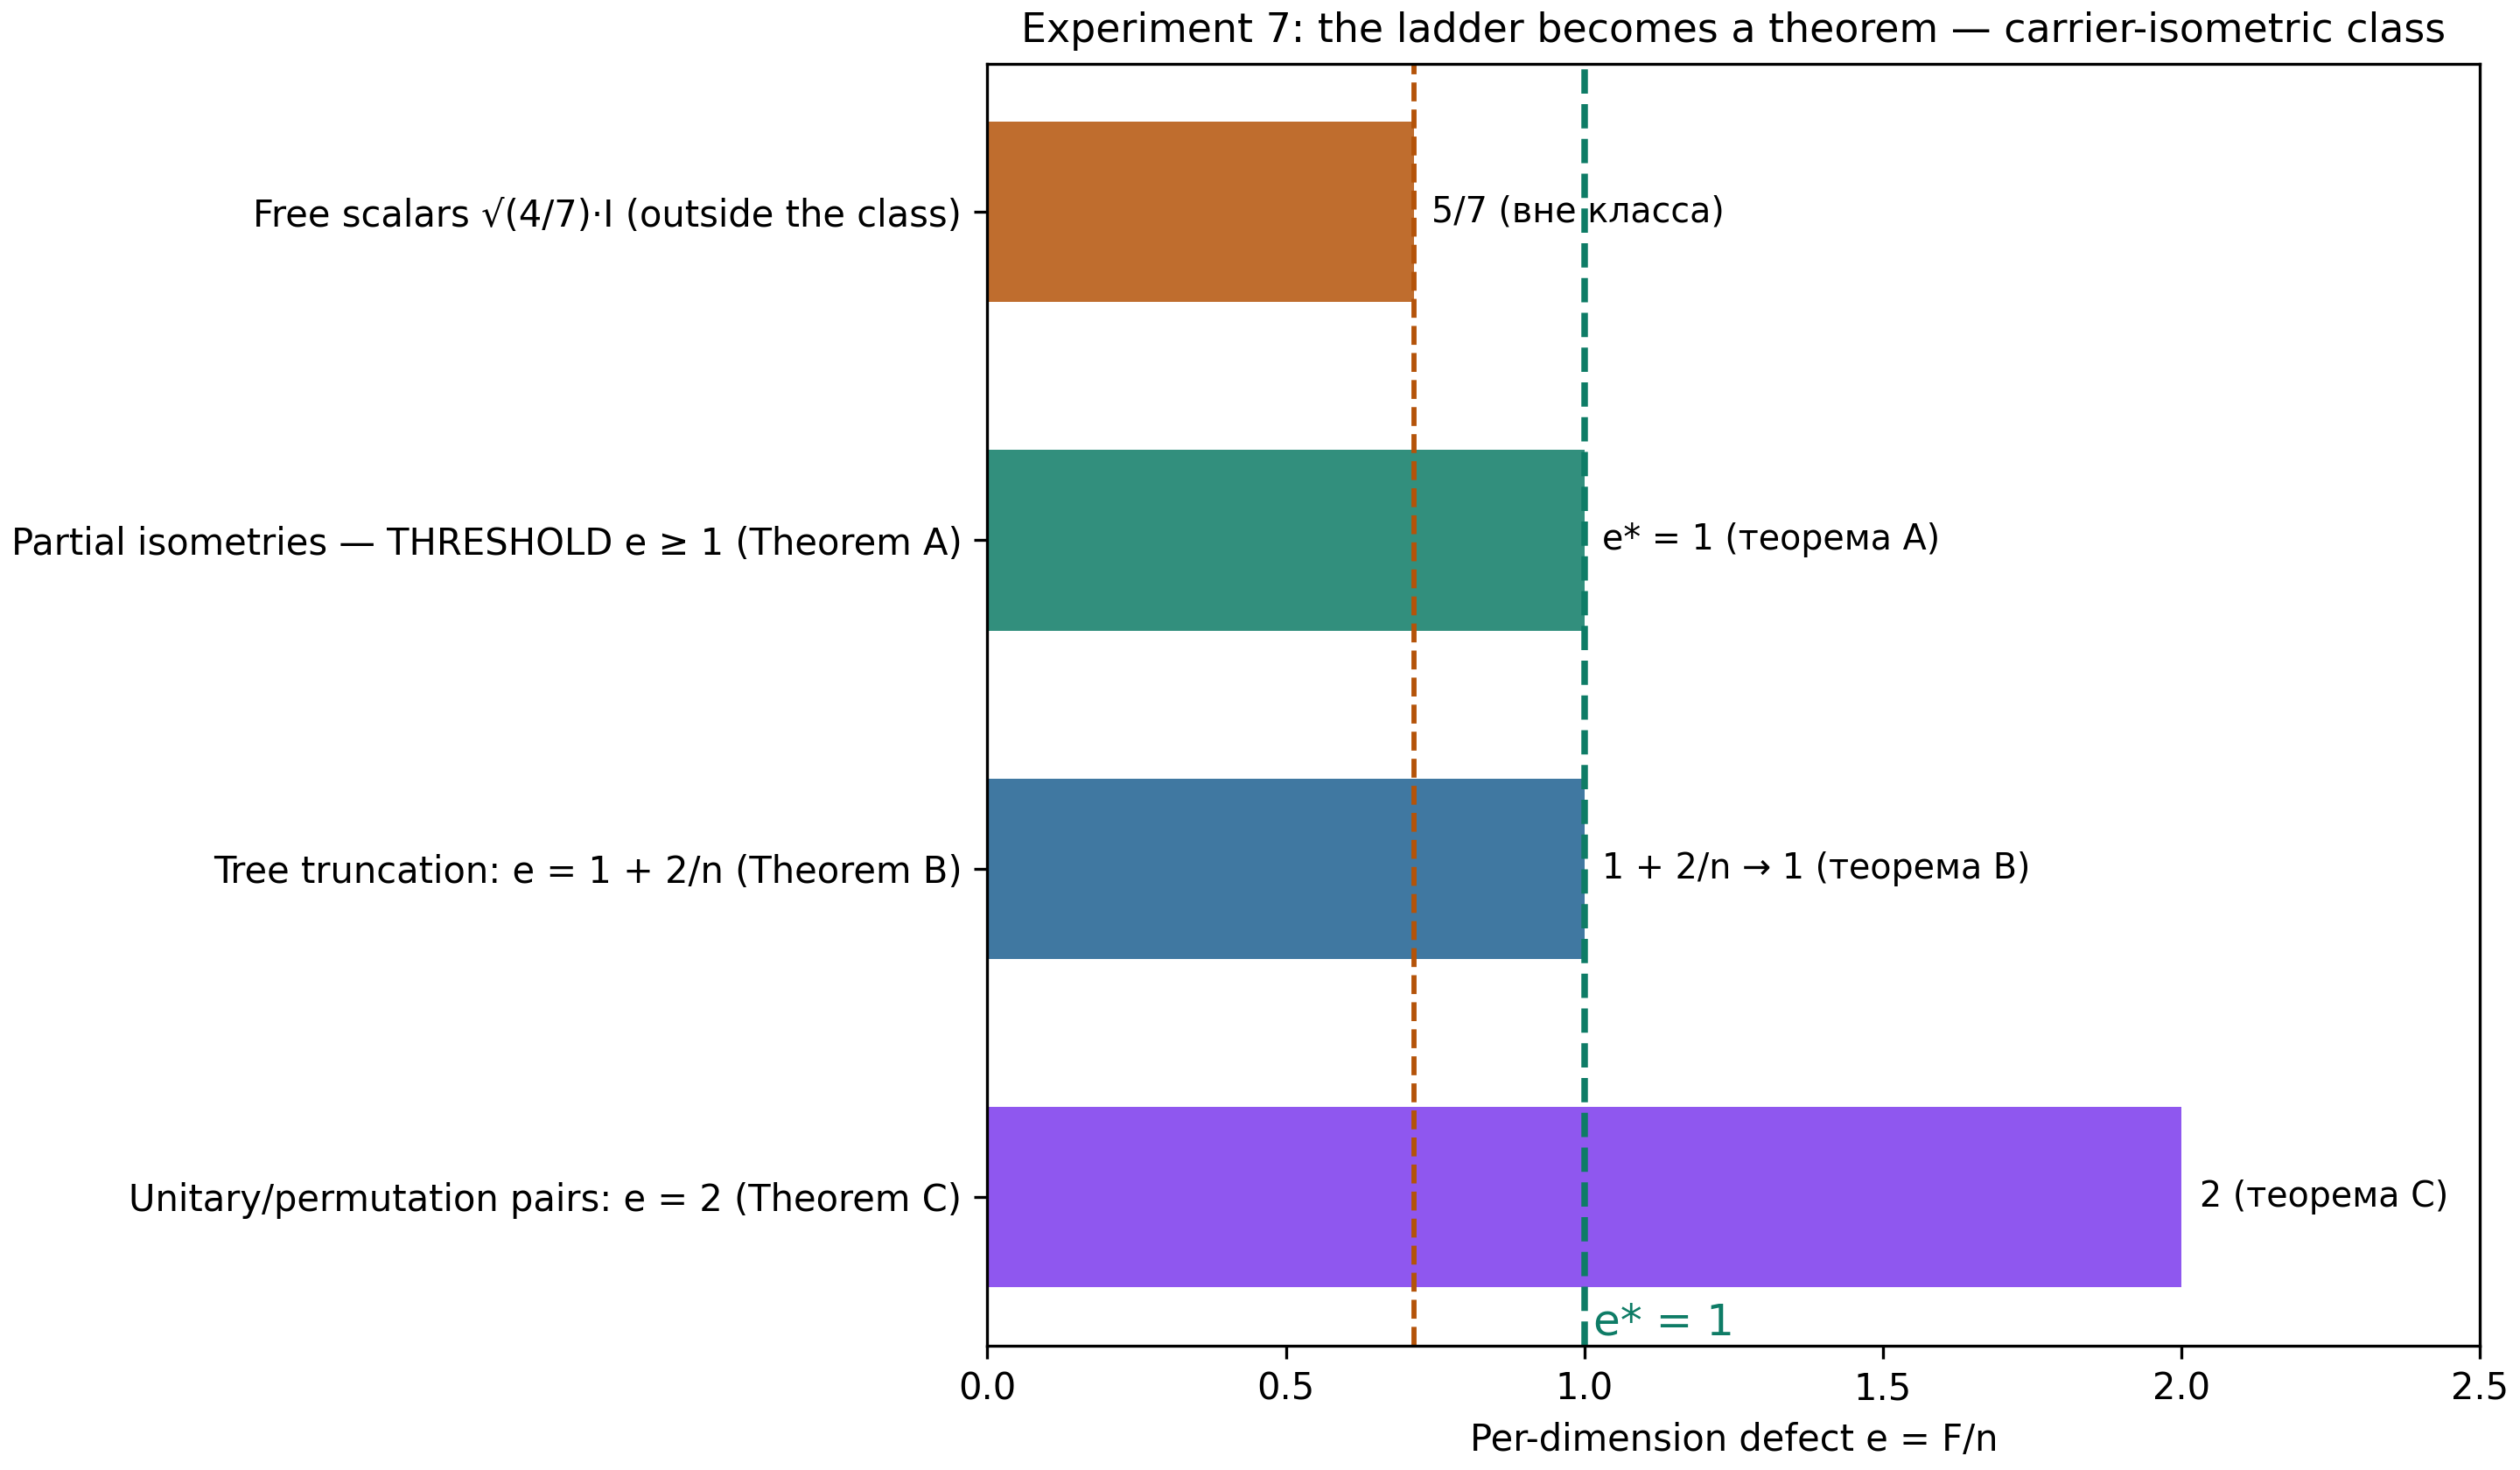
\includegraphics[width=0.82\textwidth]{figures/fig7_ladder.png}
\caption{The $e$-ladder as a theorem: the free-scalar floor $5/7$
(outside the class), theorem A ($e \ge 1$), the trimmed tree
$1 + 2/n \to 1$ (theorem B), theorem C ($e = 2$).}
\label{fig:ladder}
\end{figure}

\subsection{The sofic law is refuted}

The conjecture that natural transports of sofic data with error
$\varepsilon$ drive $e \to 0$ like $C\varepsilon^{1/2}$ is \emph{false}
in the tested class: random permutations with fixed-point share
$\varepsilon$, transported with the optimal $c$, keep the defect flat
(the Hamming scan of experiment~1). The falsifying data is committed as
an honest negative.

\section{The census attack on DSI-4}\label{sec:census}

The last empirical input of the framework is $c_{K3} =
0.04017757639214903$ (measured, audit 2026-09). The DSI-4 observation
is
\[
c_{K3} = \frac{3^3}{2^2\cdot|\mathrm{PSL}(2,7)|} = \frac{27}{672} =
\frac{9}{224} = 0.040178571428571\ldots
\]
with deviation $+0.0025\%$ --- three orders of magnitude tighter than
every structural alternative ($b_{Ch}(22)$ $+0.82\%$, braking RG
$+0.45\%$, $1/25$ $-0.44\%$).

\begin{lemma}[uniqueness]\label{lem:uniqueness}
Among fractions $p/q$ with $q \le 5000$, $p \le 32$ whose denominator
is 7-smooth within the census budget ($v_2 \le 6$, $v_3 \le 1$,
$v_7 \le 1$), the fraction $9/224$ is the only one within $0.1\%$ (a
fortiori $0.01\%$) of the measured $c_{K3}$; among the convergents of
the continued fraction of $c_{K3}$ only $1/24$ and $9/224$ pass the
census filter.
\end{lemma}

\begin{theorem}[degeneracy]\label{thm:degeneracy}
On the Hurwitz tower the two structural readings of DSI-4,
$c_I(g) = 27/(4|G|) = 9/(4V) \sim (g-1)^{-1}$ and
$c_{II}(g) = (N-1)/(F\cdot N)$, $N = 14(g-1)$, coincide \emph{only at}
$g = 3$ (the Klein quartic), while the framework branch
$c_{III}(g) = b_{Ch}(b_2(g)) \sim (g-1)^{-2}$ separates already at
$g = 7$. One DSI-amplitude measurement on any higher Hurwitz surface
discriminates the mechanisms.
\end{theorem}

\section{The two corrections: findings D1 and E1}\label{sec:findings}

\paragraph{Finding D1 (Hurwitz tower).} The repository row
$(g = 14, n = 11)$ is impossible: $84\cdot 13 = 1092$ is not divisible
by $11$, so no order-11 automorphism exists. The correct genus-14
Hurwitz group is $\mathrm{PSL}(2,13)$ of signature $(2,3,13)$; the
corrected tower
\[
(g,|G|) = (3,168)_{(2,3,7)},\ (7,504)_{(2,3,9)},\ (14,1092)_{(2,3,13)},\
(17,1344)_{(2,3,8)}
\]
passes all three checks ($84(g-1) = |G|$, $n \mid |G|$,
$1/2 + 1/3 + 1/n < 1$), and the framework curve gives
$\Delta_{Ch}(\pi/13) = 3.3672$.

\paragraph{Finding E1 (QCD centering).} The work formula
$\theta_{\mathrm{eff}} = \delta_C\, N\langle\lambda\rangle\, S_{GUE}$
requires centering: in the GUE class the semicircle is symmetric, so
$\langle\lambda\rangle = 0$ in the continuum. After centering,
$\mathrm{tr}(Q_{K3}\oplus M_F) = 32$ exactly, the $|\langle\lambda\rangle|$
scaling follows $1/\sqrt{N}$ with slope $-0.99$, and the
$\kappa_T$-sweep gives $\mathrm{BF}(\mathrm{GUE})$ up to $1165$ against
the Poisson null. The honest caveat: $V_T$ remains a constructive model
of T-violation, labeled as a hypothesis.

\begin{figure}[ht]
\centering
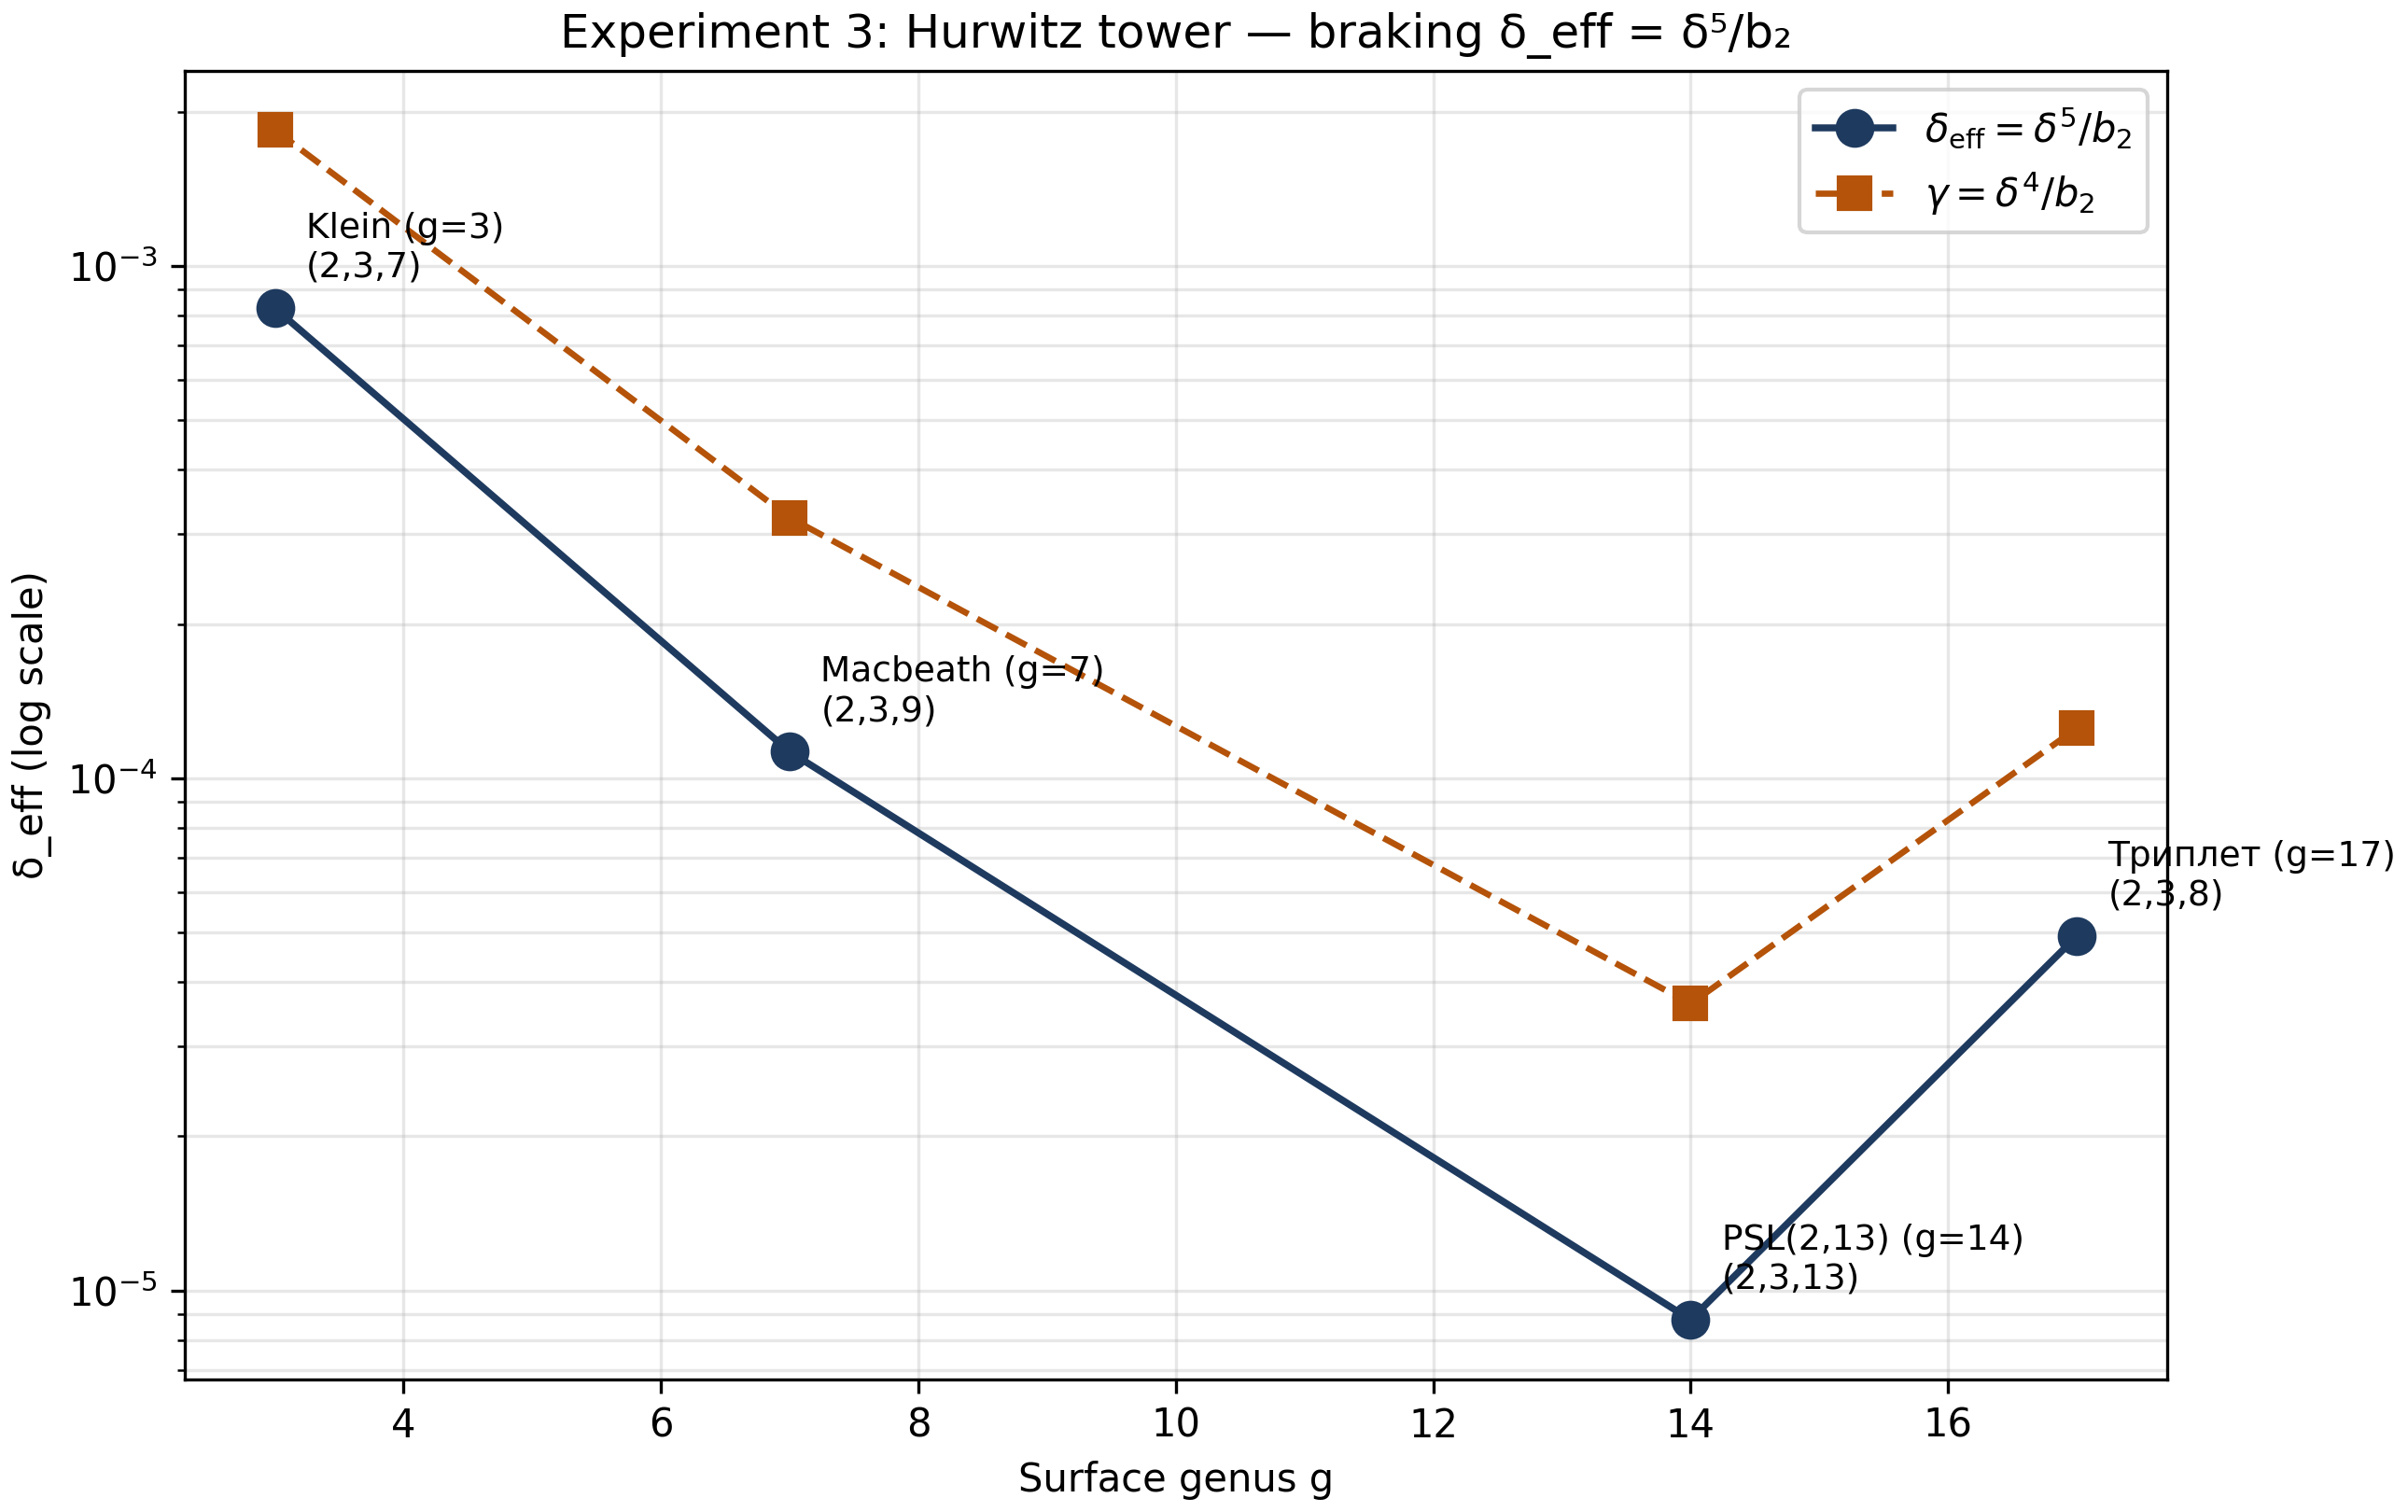
\includegraphics[width=0.8\textwidth]{figures/fig_hurwitz_tower.png}
\caption{The corrected Hurwitz tower (finding D1): the genus-14 row is
$\mathrm{PSL}(2,13)$, not the impossible $(g{=}14, n{=}11)$.}
\label{fig:hurwitz}
\end{figure}

\section{The honesty discipline}\label{sec:honesty}

Every claim of the package carries one of the labels \emph{proved}
(exact rational/integer arithmetic), \emph{verified} (machine-precision,
seeded), \emph{refuted} (kept publicly), \emph{hypothesis} (labeled
assumption) and lives in the claim ledger with the address of its
evidence. The ledger can only move one step at a time
(open $\to$ hypothesis $\to$ verified $\to$ proved), and refutations
never leave it. The reproduction contract: a fresh run must match the
committed JSONs to $10^{-10}$; any larger deviation is a finding, and
the package asks for a new ledger row rather than a re-seed.

\section{The Lean 4 layer}\label{sec:lean}

The exact stratum of the theorem layer is formalized in Lean 4 with
Mathlib (\texttt{dsi\_lab/lean4/}), sorry-free: the census arithmetic
($7F = 3V = 2E = 168$, $\chi = -4$), the continued-fraction identity
$9/224 = [0;24,1,8]$, the ladder ordering $5/7 < 1 \le 1 + 2/n \le 2$,
the scaled-permutation minimum $7(4/7)^2 - 8(4/7) + 3 = 5/7$ and the
weighted-tree value $549/49$. Theorems A/B/C are axiom-anchored: their
statements are exact, their numerical content is carried by axioms
documented with the verifying experiment, and corollary~D is derived
from theorem~A (a real proof). The axiom audit
(\texttt{DSILab\_AxiomAudit.lean}) prints the axiom footprint of every
theorem.

\section{Reproduction}\label{sec:repro}

\begin{verbatim}
cd dsi_lab
python3 -m pip install -r requirements.txt
make test          # 51+ fast theorem checks
make validate      # audit the committed verdicts
make run           # all 7 experiments, deterministic
make multilang     # C/C++/JS cross-language self-test
\end{verbatim}
Everything runs on Android/Termux unchanged. The reusable core is the
typed package \texttt{dsilab/}; the cross-language twins live in
\texttt{multilang/} (C, C++, JavaScript byte-identical; Rust, Go, Julia
sources); the monograph sources are \texttt{monograph/tex/}.

\section*{References}
\begin{enumerate}
\item R.~Fricke, F.~Klein, \emph{Vorlesungen \"{u}ber die Theorie der elliptischen Modulfunctionen}, Teubner (1897).
\item J.~Cuntz, \emph{Simple $C^*$-algebras generated by isometries}, Commun.\ Math.\ Phys.\ \textbf{57} (1977).
\item A.~Macbeath, \emph{Generators of the linear fractional groups}, Proc.\ Symp.\ Pure Math.\ \textbf{12} (1969).
\item G.~Kunze, R.~Schrader, notes on the ringdown overtone ladder and Cosmic Explorer detectability (context for the $0.84\sigma$ estimate).
\item The parent repository: \texttt{choptuik\_ac\_bc} --- the $b$--C/$a$--C framework, monographs, Einstein Direct, Collapse--Hawking Bridge, QHB, QCD Bridge.
\end{enumerate}

\end{document}
